\documentclass{llncs}
%%%%%%%%%%%%%%%%%%%%%%%%%%%%%%%%%%%%%%%%%%%%%%%%%%%%%%%%%%%
%% package sillabazione italiana e uso lettere accentate
\usepackage[italian, english]{babel}
\usepackage[utf8]{inputenc}
\usepackage[T1]{fontenc}
%%%%%%%%%%%%%%%%%%%%%%%%%%%%%%%%%%%%%%%%%%%%%%%%%%%%%%%%%%%%%

\usepackage{url}
\usepackage{xspace}
\usepackage{color}
\usepackage{listings}
\usepackage{listingsutf8}

\usepackage{manifest}

\definecolor{backcolor}{rgb}{0.988,0.988,0.988}
\definecolor{debcolor}{rgb}{0.97,1,1}
\definecolor{commentcolor}{rgb}{0,0.5,0}
\definecolor{stringcolor}{rgb}{0,0,0.8}
\definecolor{keywordcolor}{rgb}{0.7,0,0.5}
\definecolor{javagreen}{rgb}{0.25,0.5,0.35}
\definecolor{javapurple}{rgb}{0.5,0,0.35} 


\setcounter{tocdepth}{1}

%%%%%%%%%%%%%%%%%%%%%%%%%%%%%% User specified LaTeX commands.



%%%%%%%
 \newif\ifpdf
 \ifx\pdfoutput\undefined
 \pdffalse % we are not running PDFLaTeX
 \else
 \pdfoutput=1 % we are running PDFLaTeX
 \pdftrue
 \fi
%%%%%%%
 \ifpdf
 \usepackage[pdftex]{graphicx}
 \else
 \usepackage{graphicx}
 \fi
%%%%%%%%%%%%%%%
 \ifpdf
 \DeclareGraphicsExtensions{.pdf, .jpg, .tif}
 \else
 \DeclareGraphicsExtensions{.eps, .jpg}
 \fi
%%%%%%%%%%%%%%%

\newcommand{\java}{\textsf{Java}}
\newcommand{\android}{\texttt{Android}}
\newcommand{\dsl}{\texttt{DSL}}
\newcommand{\jazz}{\texttt{Jazz}}
\newcommand{\rtc}{\texttt{RTC}}
\newcommand{\ide}{\texttt{Contact-ide}}
\newcommand{\xtext}{\texttt{XText}}
\newcommand{\xpand}{\texttt{Xpand}}
\newcommand{\xtend}{\texttt{Xtend}}
\newcommand{\pojo}{\texttt{POJO}}
\newcommand{\junit}{\texttt{JUnit}}

\newcommand{\action}[1]{\texttt{#1}\xspace}
\newcommand{\codescript}[1]{{\scriptsize{\texttt{#1}}}\xspace}
\newcommand{\code}[1]{{\color{blue}\small{\texttt{#1}}}}
\newcommand{\fname}[1]{\small{\color{magenta}\texttt{#1}}}
\newcommand{\node}{\textsf{NodeJs}}
\newcommand{\qa}{\textsf{\textit{QActor}}}

% Cross-referencing
\newcommand{\labelsec}[1]{\label{sec:#1}}
\newcommand{\xs}[1]{\sectionname~\ref{sec:#1}}
\newcommand{\xsp}[1]{\sectionname~\ref{sec:#1} \onpagename~\pageref{sec:#1}}
\newcommand{\labelssec}[1]{\label{ssec:#1}}
\newcommand{\xss}[1]{\subsectionname~\ref{ssec:#1}}
\newcommand{\xssp}[1]{\subsectionname~\ref{ssec:#1} \onpagename~\pageref{ssec:#1}}
\newcommand{\labelsssec}[1]{\label{sssec:#1}}
\newcommand{\xsss}[1]{\subsectionname~\ref{sssec:#1}}
\newcommand{\xsssp}[1]{\subsectionname~\ref{sssec:#1} \onpagename~\pageref{sssec:#1}}
\newcommand{\labelfig}[1]{\label{fig:#1}}
\newcommand{\xf}[1]{\figurename~\ref{fig:#1}}
\newcommand{\xfp}[1]{\figurename~\ref{fig:#1} \onpagename~\pageref{fig:#1}}
\newcommand{\labeltab}[1]{\label{tab:#1}}
\newcommand{\xt}[1]{\tablename~\ref{tab:#1}}
\newcommand{\xtp}[1]{\tablename~\ref{tab:#1} \onpagename~\pageref{tab:#1}}
% Category Names
\newcommand{\sectionname}{Section}
\newcommand{\subsectionname}{Subsection}
\newcommand{\sectionsname}{Sections}
\newcommand{\subsectionsname}{Subsections}
\newcommand{\secname}{\sectionname}
\newcommand{\ssecname}{\subsectionname}
\newcommand{\secsname}{\sectionsname}
\newcommand{\ssecsname}{\subsectionsname}
\newcommand{\onpagename}{on page}

\newcommand{\xauthA}{Luca Bonfiglioli}
\newcommand{\xauthB}{Nicola Fava}
\newcommand{\xauthC}{Antonio Grasso}
\newcommand{\xemailauthA}{\email{luca.bonfiglioli10@studio.unibo.it}}
\newcommand{\xemailauthB}{\email{nicola.fava@studio.unibo.it}}
\newcommand{\xemailauthC}{\email{antonio.grasso5@studio.unibo.it}}
\newcommand{\xfaculty}{II Faculty of Engineering}
\newcommand{\xunibo}{Alma Mater Studiorum -- University of Bologna}
\newcommand{\xaddrBO}{viale Risorgimento 2}
\newcommand{\xaddrCE}{via Venezia 52}
\newcommand{\xcityBO}{40136 Bologna, Italy}
\newcommand{\xcityCE}{47023 Cesena, Italy}

%
% Comments
%
\newcommand{\todo}[1]{\bf{TODO:}\emph{#1}}


\renewcommand{\lstlistingname}{Listato}
\lstset{ 
	backgroundcolor=\color{backcolor},
	basicstyle=\small\ttfamily,
	breakatwhitespace=false,
	breaklines=true,
	captionpos=b,                    
  	commentstyle=\color{javagreen}, 
	frame=single,	                   
	keepspaces=true,
	keywordstyle=\color{javapurple}\bfseries,
	language=Java,
	morekeywords={System, Event, Context, ip, host, port, QActor, context, Plan, normal, swtichTo, transition, stopAfter, whenEvent, finally, repeatPlan, resumeLastPlan, onEvent, Dispatch, whenMsg, onMsg, onEvent, EventHandler, println, switchTo, javaRun, forwardEvent, emit, printCurrentMessage, delay, printCurrentEvent, forward},
	numbers=left,
	numberstyle=\tiny,
	rulecolor=\color{black},
	showspaces=false,
	showstringspaces=false,
	showtabs=false
	stepnumber=1,
	stringstyle=\color{stringcolor},
	tabsize=2,
	inputencoding=utf8/latin1,
	caption=\lstname	% to use with \lstinputlisting
}



\begin{document}

\title{Software Engineering process}

\author{\xauthA , \xauthB, \xauthC}

\institute{%
  \xunibo\\
  \xaddrBO, \xcityBO\\
  \xemailauthA\\
  \xemailauthB\\
  \xemailauthC
}

\maketitle
\newpage
\tableofcontents
\newpage

%\begin{abstract}
%\footnotesize
%\keywords{
%Software engineering, software development process, process representation, .... }
%\end{abstract}

%\sloppy

%===========================================================================
%\section{Introduction}
\section{Introduzione}
\labelsec{intro}

%===========================================================================
%
%===========================================================================
\section{Vision}
\labelsec{vision}

%===========================================================================
% 
%===========================================================================
%\section{Requirements}
\section{Requisiti}
\labelsec{Requirements}
Nella casa di una determinata città (per esempio Bologna), viene usato un \action{ddr} robot per pulire il pavimento di una stanza (\code{R-FloorClean}).
Il pavimento della stanza è piatto ed è costituito di un materiale solido; è inoltre equipaggiato con due \textit{sonar}, chiamati \code{sonar1} e \code{sonar2}, come mostrato in Figura \ref{fig:virtualrobot} (\code{sonar1} è quello mostrato in alto). La posizione iniziale (\code{start-point}) del robot è riconosciuta da \code{sonar1}, mentre la posizione finale (\code{end-point}) dal \code{sonar2}.

Il robot lavora secondo le seguenti condizioni:
\begin{enumerate}
\item \code{R-Start}: un utente autorizzato (\code{authorized user}) ha inviato un comando \action{START} usando una interfaccia \action{GUI} (\code{console}) in esecuzione su un normale \action{PC} oppure su uno smart device (\action{Android}).
\item \code{R-TempOk}: il valore di temperatura nella città non è superiore ad un limite prefissato (per esempio 25\,$^{\circ}$C).
\item \code{R-TimeOk}: l'orario corrente è all'interno di un intervallo dato (per esempio fra le 7 e le 10).
\end{enumerate}

Mentre il robot è in movimento:
\begin{itemize}
\item se il robot è \fname{real}, un \action{Led} posto su di esso deve lampeggiare (\code{R-BlinkLed});
\item se il robot è \fname{virtual}, una \action{Led Hue Lamp} disponibile nella casa deve lampeggiare (\code{R-BlinkHue});
\item deve evitare gli ostacoli fissi (per esempio i mobili) presenti nella stanza (\code{R-AvoidFix}) e/o gli ostacoli mobili come palloni, gatti, ecc. (\code{R-AvoidMobile}).
\end{itemize}

Inoltre il robot deve interrompere la sua attività quando è verificata una delle seguenti condizioni:
\begin{enumerate}
\item \code{R-Stop}: un utente autorizzato ha inviato il comando di \action{STOP} utilizzando la \code{console}.
\item \code{R-TempKo}: il valore di temperatura della città diventa più alto del valore prefissato.
\item \code{R-TimeKo}: l'orario corrente non è più all'interno dell'intervallo prefissato.
\item \code{R-Obstacle}: il robot ha trovato un ostacolo che non è in grado di superare.
\item \code{R-End}: il robot ha finito il suo lavoro.
\end{enumerate}

Durante il suo funzionamento il robot può:
\begin{itemize}
\item \code{R-Map}: costruire una mappa del pavimento della stanza con la posizione degli ostacoli fissi. Una volta ottenuta, la mappa può essere utilizzata per definire un percorso (ottimo) dallo \code{start-point} all'\code{end-point}.
\end{itemize}

\begin{figure}
\centering
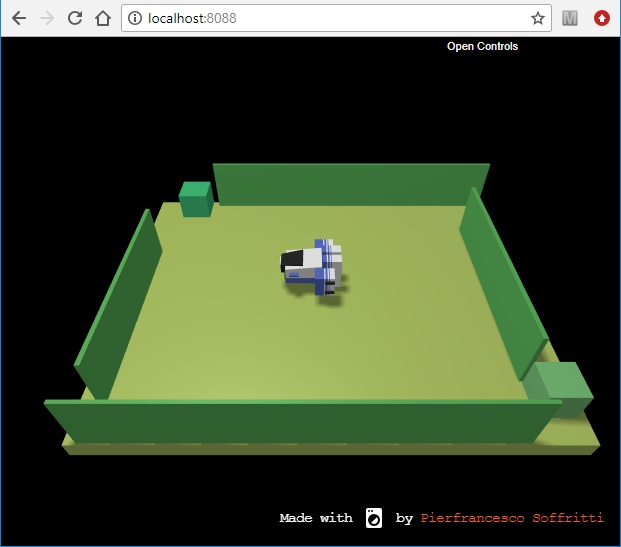
\includegraphics[scale=0.7]{img/virtualRobot.jpg}
\caption{Esempio di pavimento con il robot in ambiente simulato}
\label{fig:virtualrobot}
\end{figure}

%===========================================================================
%
%===========================================================================
%\section{Requirement analysis}
\section{Analisi dei requisiti}
\labelsec{ReqAnalysis}
Il sistema da modellare sarà, come esplicitato dai requisiti, eterogeneo e distribuito, in particolare composto da almeno due nodi: il nodo "Robot" e il nodo "PC / Android". 
Per la modellazione si utilizza il linguaggio \qa\ in quanto adatto alla modellazione di sistemi distribuiti.

Prima di formalizzare il contenuto del diagramma di  \ref{fig:reqAnalysis}, ci soffermiamo sul significato di ciascun elemento. 

Il primo dei due nodi che abbiamo modellato è il nodo "PC / Android" che si occupa di mostrare la \action{GUI} e interagire direttamente con un utente umano, richiedendone l'autenticazione. Come da requisito \code{R-Start} l'interfaccia utente deve poter essere utilizzabile sia su \action{PC} che su un dispositivo \action{Android}, tuttavia, essendo le funzioni che essa deve svolgere identiche in entrambi i casi, abbiamo rappresentato entrambi i nodi come uno unico. Su questo nodo esegue l'attore "GUI/Authenticator", che consente all'utente di autenticarsi e inviare i comandi di \action{START} e \action{STOP} al robot (\code{R-Start} e \code{R-Stop}). 

Il secondo nodo "Raspberry / PC" controlla il robot, esso può essere in esecuzione su un PC, nel caso del robot virtuale, oppure su un Raspberry Pi nel caso del robot reale. L'attore "Robot" si pone in attesa dei comandi inviati da "GUI/Authenticator" e riceve informazioni sull'ambiente esterno da un sensore di temperatura e un timer (\code{R-TempOk}, \code{R-TimeOk}, \code{R-TempKo}, \code{R-TimeKo}). Durante l'esecuzione, in caso di movimento, l'attore "Robot" invia a "Led" e a "Hue Lamp" comandi per l'accensione e lo spegnimento (\code{R-BlinkLed}, \code{R-BlinkHue}). 

L'attore "Robot" si occupa inoltre di gestire la logica applicativa, ovvero, in seguito alla ricezione del comando \action{START} da parte dell'utente, prendere decisioni circa il movimento del robot all'interno della stanza – per il robot reale – e all'interno dell'ambiente simulato – per il robot virtuale -, tentando di evitare gli ostacoli fissi e mobili (\code{R-AvoidFix}, \code{R-AvoidMobile}), costruendo una mappa (\code{R-Map}) dell'ambiente.

Se l'attore "Robot" trova un ostacolo che non riesce ad evitare si deve fermare (\code{R-Obstacle}).
Questa situazione si verifica quando il robot trova uno o più ostacoli che gli impediscono di avanzare in una direzione diversa da quella da cui è arrivato.

\begin{figure}
\centering
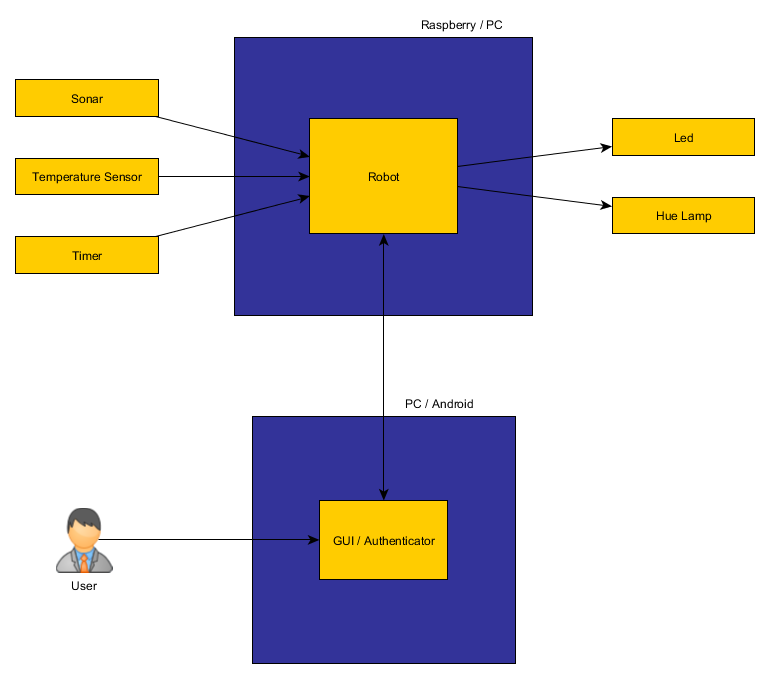
\includegraphics[scale=0.4]{img/requirements_analysis.png}
\caption{Analisi dei requisiti informale}
\label{fig:reqAnalysis}
\end{figure}

\lstinputlisting[label={lst:reqAnalysisRobot}]{code/reqAnalysisRobot.qa}
\lstinputlisting[label={lst:reqAnalysisUser}]{code/reqAnalysisUser.qa}


%===========================================================================
%
%===========================================================================
%\section{Problem analysis}
\section{Analisi del problema}
\labelsec{ProblemAnalysis}
Il primo problema che sorge è quello di stabilire quale nodo si occuperà di autenticare l'utente. Una possibilità è che sia sul nodo del robot: in questo caso il robot potrebbe non disporre delle adeguate risorse computazionali per gestire il processo di autenticazione, tuttavia questo garantirebbe maggiore sicurezza. Un'altra possibilità è che l'autenticazione sia su un nodo diverso rispetto a quello del robot: ciò consente di non utilizzare le risorse computazionali del robot richiedendo però maggiori accortezze sulla sicurezza. In quest'ultimo caso l'autenticazione potrebbe essere gestita dal nodo dell'utente oppure da un nodo distinto, il quale comporterebbe costi maggiori.

Un altro problema è quello dell'interfaccia \action{GUI}, che deve poter eseguire su dispositivi eterogenei. A tal proposito, una possibilità sarebbe creare client nativi per ogni piattaforma con costi elevati oppure più semplicemente utilizzare una pagina web. 

La comunicazione tra utente e robot tramite \action{GUI} può avvenire via messaggi o via eventi. La comunicazione ad eventi permette di disaccoppiare \action{GUI} e robot, consentendo di utilizzare un'unica \action{GUI} per comunicare con diversi robot. Utilizzando gli eventi può essere adottato un approccio \code{event-based} o un approccio \code{event-driven}. Nell'approccio \code{event-based} il robot non sarebbe sempre sensibile agli eventi, potendone perdere alcuni. Al contrario, nell'approccio \code{event-driven} il robot sarebbe sempre sensibile agli eventi perdendo tuttavia reattività.
\\

\lstinputlisting[label={lst:probAnalysisRobot}]{code/probAnalysisRobot.qa}
\lstinputlisting[label={lst:probAnalysisUser}]{code/probAnalysisUser.qa}

%===========================================================================
%
%===========================================================================
%\section{Project}
\section{Progettazione}
\labelsec{Project}
%===========================================================================
%
%===========================================================================
%\section{Implementation}
\section{Implementazione}
\labelsec{Implementation}
%===========================================================================
%
%===========================================================================
%\section{Testing}
\labelsec{Testing}
%===========================================================================
%
%===========================================================================
%\section{Maintenance}
\labelsec{Maintenance}
%===========================================================================
%
%===========================================================================
%\section{Deployment}
\labelsec{Deployment}
%
%===========================================================================
\newpage
%\section{Authors}
\section{Autori}
\labelsec{Authors}
%===========================================================================

\vskip.5cm
%
% I nostri nomi sono authA, authB, authC in ordine alfabetico.
%
\begin{table}
\begin{tabular}{|c|c|c|}
\hline
\multicolumn{3}{|c|}{Foto degli autori} 
\\
\hline
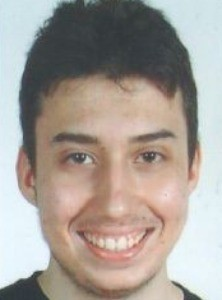
\includegraphics[scale = 0.4]{img/foto_authA.jpg}&
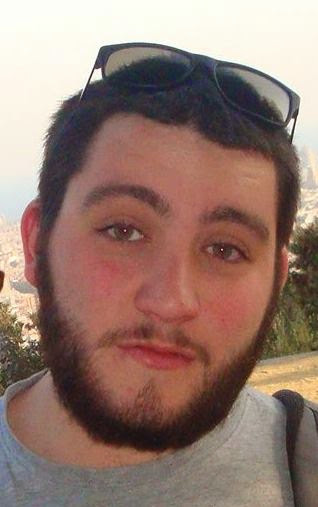
\includegraphics[scale = 0.26]{img/foto_authB.jpg}&
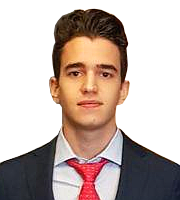
\includegraphics[scale = 1.0]{img/foto_authC.png}
\\
\hline
\xauthA& \xauthB& \xauthC
\\
\hline
\end{tabular}
\end{table}



\end{document}












